\documentclass{article}
\author{Huang Hsin}

\usepackage[english]{babel}
\usepackage[letterpaper,top=2cm,bottom=2cm,left=3cm,right=3cm,marginparwidth=1.75cm]{geometry}

\usepackage{cite}
\usepackage{amsmath}
\usepackage{amsthm}
\usepackage{amssymb}
\usepackage{array}
\usepackage{graphicx}
\usepackage{subcaption}
\usepackage{algpseudocode}
\usepackage{algorithm}
\usepackage[colorlinks=true, allcolors=blue]{hyperref}
\renewcommand{\theenumi}{(\Alph{enumi})}

\usepackage{graphicx}
\graphicspath{ {../result_images/} }

\newtheorem{proposition}{Proposition}[section]
\newtheorem{assumption}{Assumption}[section]
\newtheorem{theorem}{Theorem}
\newtheorem{definition}{Definition}

% 

\title{Research note}

\begin{document}
\maketitle

\begin{abstract}
This is a research note for implementing quasi-Newton method on minimax problem.
\end{abstract}

\section{Introduction}

\section{Preliminary}

We focus on the nonconvex-nonconcave minimax problem:
\begin{equation}
    \min_{x \in \mathbb{R}^n} \max_{y \in \mathbb{R}^m} f(x,y)
\end{equation}
where $f: \mathbb{R}^{n+m} \to \mathbb{R}$ is twice continuously differentiable, i.e. $f \in \mathcal{C}^2$. Here, we define the local optimal solution of this problem as follow:
\begin{definition}[strict local minimax(SLmM), \cite{evtushenko1974minimax}]
    $(x^*, y^*)$ is a strict local minimax point (SLmM) of a twice differentiable function $f$ if it is a stationary point, $\partial_{yy}f(x^*,y^*) \prec 0$ and $\mathbf{D}_{xx}f(x^*,y^*) \succ 0$
\end{definition}

Such definition has appeared in many research focusing on local convergence of minimax problem.

Now, we seperate the problem into two subproblem, the inner problem solving $\Phi(x) = \max_{y \in \mathbb{R}^m}f(x,y)$ and the outer problem solving $\min_{x \in \mathbb{R}^n} \Phi(x)$.

\subsection{Inner problem}
\label{InnerProblem}
For the inner problem, which is a simple one-variable maximization problem $\max_{y \in \mathbb{R}^m}f(x,y)$ where the $x$ is fixed. There are already many well-known solutions for this kind of problem.
Such as gradient ascent:
\begin{equation}
    y_{i+1} = y_i + \alpha_i \partial_y f(x, y_i)
\end{equation}
or Newton method:
\begin{equation}
    y_{i+1} = y_i - \alpha_i (\partial_{yy} f(x, y_i))^{-1}\partial_y f(x, y_i)
\end{equation}
Idealy, we want to solve the inner problem accurately to give a precise function $\Phi(x)$ to the outer problem.
However, in practice, it is time consuming to solve inner problem precisely.
Therefore, instead of solving the inner problem exactly, we run several update to get the approximation of function $\Phi$.

\subsection{Outer problem}
\label{OuterProblem}
For the outer problem $\min_{x \in \mathbb{R}^n} \Phi(x)$, since we are not minimizing the fucntion $f$ directly, we need to analyze the function $\Phi(x) = \max_{y \in \mathbb{R}^m} f(x, y)$ furthermore.

At a SLmM $(x^*, y^*)$, We know that $\partial_yf(x^*,y^*(x)) = 0$ and $\partial_{yy}f(x^*, y^*) \prec 0$ by definition.
By implict theorem, we know that there are neighborhoods $\mathcal{N}(x^*) \subset \mathbb{R}^n$, $\mathcal{N}(y^*) \subset \mathbb{R}^m$ and a continuously differentiable function
\begin{equation}
    r: \mathcal{N}(x^*) \to \mathcal{N}(y^*) \text{ s.t. } \partial_y f(x, r(x)) = 0
\end{equation}
where $r(x)$ is a local minimizer of $f(x, \cdot)$ and $\Phi(x) = f(x, r(x))$. Therefore, on $\mathcal{N}(x^*)$:
\begin{equation}
    \nabla \Phi(x) = \partial_xf(x, r(x)) + \nabla r(x) \partial_yf(x, r(x)) = \partial_xf(x, r(x))
\end{equation}
For the second derivative $\nabla^2\Phi(x)$.
Since $\partial_yf(x, r(x)) = 0$, we know that
\begin{flalign*}
    &\partial_{xy} f(x, r(x)) + \nabla r(x) \partial_{yy}f(x,r(x)) = 0 \\
    &\nabla y^*(x) = -\partial_{xy}f(x, y^*(x)) (\partial_{yy}f(x, y^*(x)))^{-1}
\end{flalign*}
From $\nabla \Phi(x) = \partial_xf(x, y^*(x))$, we know that 
\begin{flalign}
    \label{eq3}
    \nabla^2\Phi(x) &= \partial_{xx}f(x, y^*(x)) + \nabla y^*(x) \partial_{yx} f(x, y^*(x)) \nonumber\\ 
                    &= \partial_{xx}f(x, y^*(x)) - \partial_{xy}f(x, y^*(x))(\partial_{yy}f(x, y^*(x)))^{-1}\partial_{yx}f(x, y^*(x))
\end{flalign}
By using \hyperref[eq3]{equation 3}, the Newton update will be:
\begin{equation}
    x^{k+1} = x^k - (\nabla^2 \Phi(x^k))^{-1}\nabla\Phi(x^k)
\end{equation}

\section{Quasi-Newton method}
Since calculating the Hessian used in Newton method might be time consuming and gradient descent(ascent) converge slowly,
we can try to use quasi-Newton method.
Quasi-Newton method is a set of methods that approximate the Hessian by using only gradient to avoid expensive computation.
As we discussed in section \hyperref[InnerProblem]{2.1}, we can use the normal quasi-Newton method directly on the inner problem:
\begin{equation}
    y_{i+1} = y_i + \alpha_i H_i \partial_y f(x, y_i)
\end{equation}
where $H_i$ is the approximation of the inverse of Hessian. Notice that we use the subscript $i$ rather than $k$ since if we set $H_0 = I$ and run the update only once, then it will be a simple gradient ascent step.
Therefore, we will run the quasi-Newton step several time to let the approximation of Hessian become more accurate.\\
For outer problem, 
\begin{equation}
    x^{k+1} = x^k - B(x^k)^{-1}\nabla\Phi(x^k) = x^k - H(x^k)\nabla\Phi(x^k)
\end{equation}
where $B(x)$ is the approximate Hessian and $H(x)$ is the inverse of approximate Hessian.

Here, we have many option for the approximation such as BFGS.\\
In normal BFGS for a minimization problem $\min z(x)$, we approximate the Hessian by the step difference $s$ and the gradient difference $g$.
\begin{equation}
    H_{k+1} = (I - \frac{s_k g_k^T}{g_k^T s_k})H_k(I - \frac{g_k s_k^T}{g_k^T s_k}) + \frac{s_k s_k^T}{g_k^T s_k},\; s_k = x_{k+1} - x_k,\; g_k = \nabla z_{k+1} - \nabla z_k
\end{equation}
Come back to the minimax problem. For the inner problem, we are simply doing a maximize version quasi-Newton method since we are maximizing a function $\max_{y \in \mathbb{R}^m} f(x,y)$.
For the outer problem, we are doing $\min_{x \in \mathbb{R}^n} \Phi(x)$, so we use the gradient $\nabla\Phi(x) = \partial_xf(x, y^*(x))$ in our gradient step.

\section{Algorithm}
Algorithm \hyperref[GDBFGS]{1} is gradient-descent-BFGS(GD-BFGS) where we use gradient descent for outer problem and BFGS for inner problem.
\begin{algorithm}
    \caption{Gradient-descent-BFGS}
    \label{GDBFGS}
    \begin{algorithmic}
        \State (step size $\alpha_x, \alpha_y$, initialization $x_0$, $y_0$)
        \State $\textbf{GDBFGS}(\alpha_x, \alpha_y, x_0, y_0)$:
        \For{$k=0,1,2,3...$}
        \State $x_{k+1} \gets \alpha_x \partial_xf(x_k, y_k)$
        \State $y_{k+1} \gets \textbf{InnerBFGS} (\alpha_y, x_{k+1}, y_k)$
        \EndFor\\
        \Return $x_k, y_k$
    \end{algorithmic}
\end{algorithm}
\begin{algorithm}
    \caption{InnerBFGS}
    \label{InnerBFGS}
    \begin{algorithmic}
        \State $\textbf{InnerBFGS}(\alpha_y, x, y)$:
        \State $H_0 \gets I$, $y_0 \gets y$
        \For{$i=0,1,2,3...$}
            \State $s_i \gets \alpha_x H_k \partial_y f(x, y_i)$
            \State $y_{i+1} \gets y_i + s_i$
            \State $g_i \gets - \partial_y f(x, y_{i+1}) + \partial_y f(x, y_i)$
            \State $H_{i+1} \gets (I - \frac{s_i g_i^T}{g_i^T s_i})H_i(I - \frac{g_i s_i^T}{g_i^T s_i}) + \frac{s_is_i^T}{g_i^T s_i}$
        \EndFor\\
        \Return $y_i$
    \end{algorithmic}
\end{algorithm}
\\Algorithm \hyperref[CBFGS]{3} is complete-BFGS(CBFGS) where we use BFGS for both outer and inner problem. Notice that Algorithm \hyperref[GDBFGS]{1} and \hyperref[CBFGS]{3} share the same inner loop (Algorithm \hyperref[InnerBFGS]{2}).
\begin{algorithm}
    \caption{Complete-BFGS}
    \label{CBFGS}
    \begin{algorithmic}
        \State (step size $\alpha_x, \alpha_y$, initialization $x_0$, $y_0$)
        \State $\textbf{CBFGS}(\alpha_x, \alpha_y, x_0, y_0)$:
        \State $H_0 \gets I$
        \For{$k=0,1,2,3...$}
            \State $s_k = - \alpha_x H_k \partial_x f(x_k, y_k)$
            \State $x_{k+1} = x_k + s_k$
            \State $g_k = \partial_x f(x_{k+1}, y_k) - \partial_x f(x_k, y_k)$
            \State $H_{k+1} = (I - \frac{s_k g_k^T}{g_k^T s_k})H_k(I - \frac{g_k s_k^T}{g_k^T s_k}) + \frac{s_ks_k^T}{g_k^T s_k}$
            \State $y_{k+1} = \textbf{InnerLoop} (x_{k+1}, y_k)$
        \EndFor\\
        \Return $x_k,y_k$
    \end{algorithmic}
\end{algorithm}

\section{Experiment}

For the experiment, we run well-conditioned guassian mean estimation, ill-conditioned guassian mean estimation and
ill-conditioned gaussian covariance estimation.

\begin{table}[h!]
    \centering
    \begin{tabular}{|c|>{\centering\arraybackslash}p{3.5cm}|>{\centering\arraybackslash}p{3.5cm}|>{\centering\arraybackslash}p{3.5cm}|}
        \hline
        algorithm & mean & mean(ill conditioned) & covariance \\ \hline
        GDA    & 139.4 (0.05, 0.5, 1)  & 138.6 (0.05, 0.5, 1)  & 146.9 (0.02, 0.2, 1)  \\ \hline
        GDN    & 151.3 (0.05, 1.0, 1)  & 150.3 (0.05, 1.0, 1)  & 217.0 (0.02, 1.0, 1)  \\ \hline
        GDBFGS & 151.6 (0.05, 1.0, 10) & 147.2 (0.05, 1.0, 10) & 176.5 (0.02, 1.0, 10) \\ \hline
        CN     & 177.9 (1.0 , 1.0, 1)  & 173   (1.0 , 1.0, 1)  & 314   (1.0 , 1.0, 10) \\ \hline
        CBFGS  & 142.9 (0.5 , 1.0, 10) & 144   (0.5 , 1.0, 10) & 198.0 (0.5 , 1.0, 20) \\ \hline
        BFGSN  & 150.0 (0.5 , 1.0, 1)  & 146.4 (0.5 , 1.0, 1)  & 211.5 (0.7 , 1.0, 1)  \\ \hline
    \end{tabular}
    \caption{Time spent for different model and algorithm(unit: second per 1000 epochs). \\ Note: the numbers brackets are $\alpha_x, \alpha_y, \text{\# of inner loop}$}
    \label{tab:sample}
\end{table}

\begin{figure}[htbp]
    \centering
    \begin{subfigure}[b]{0.45\textwidth}
        \centering
        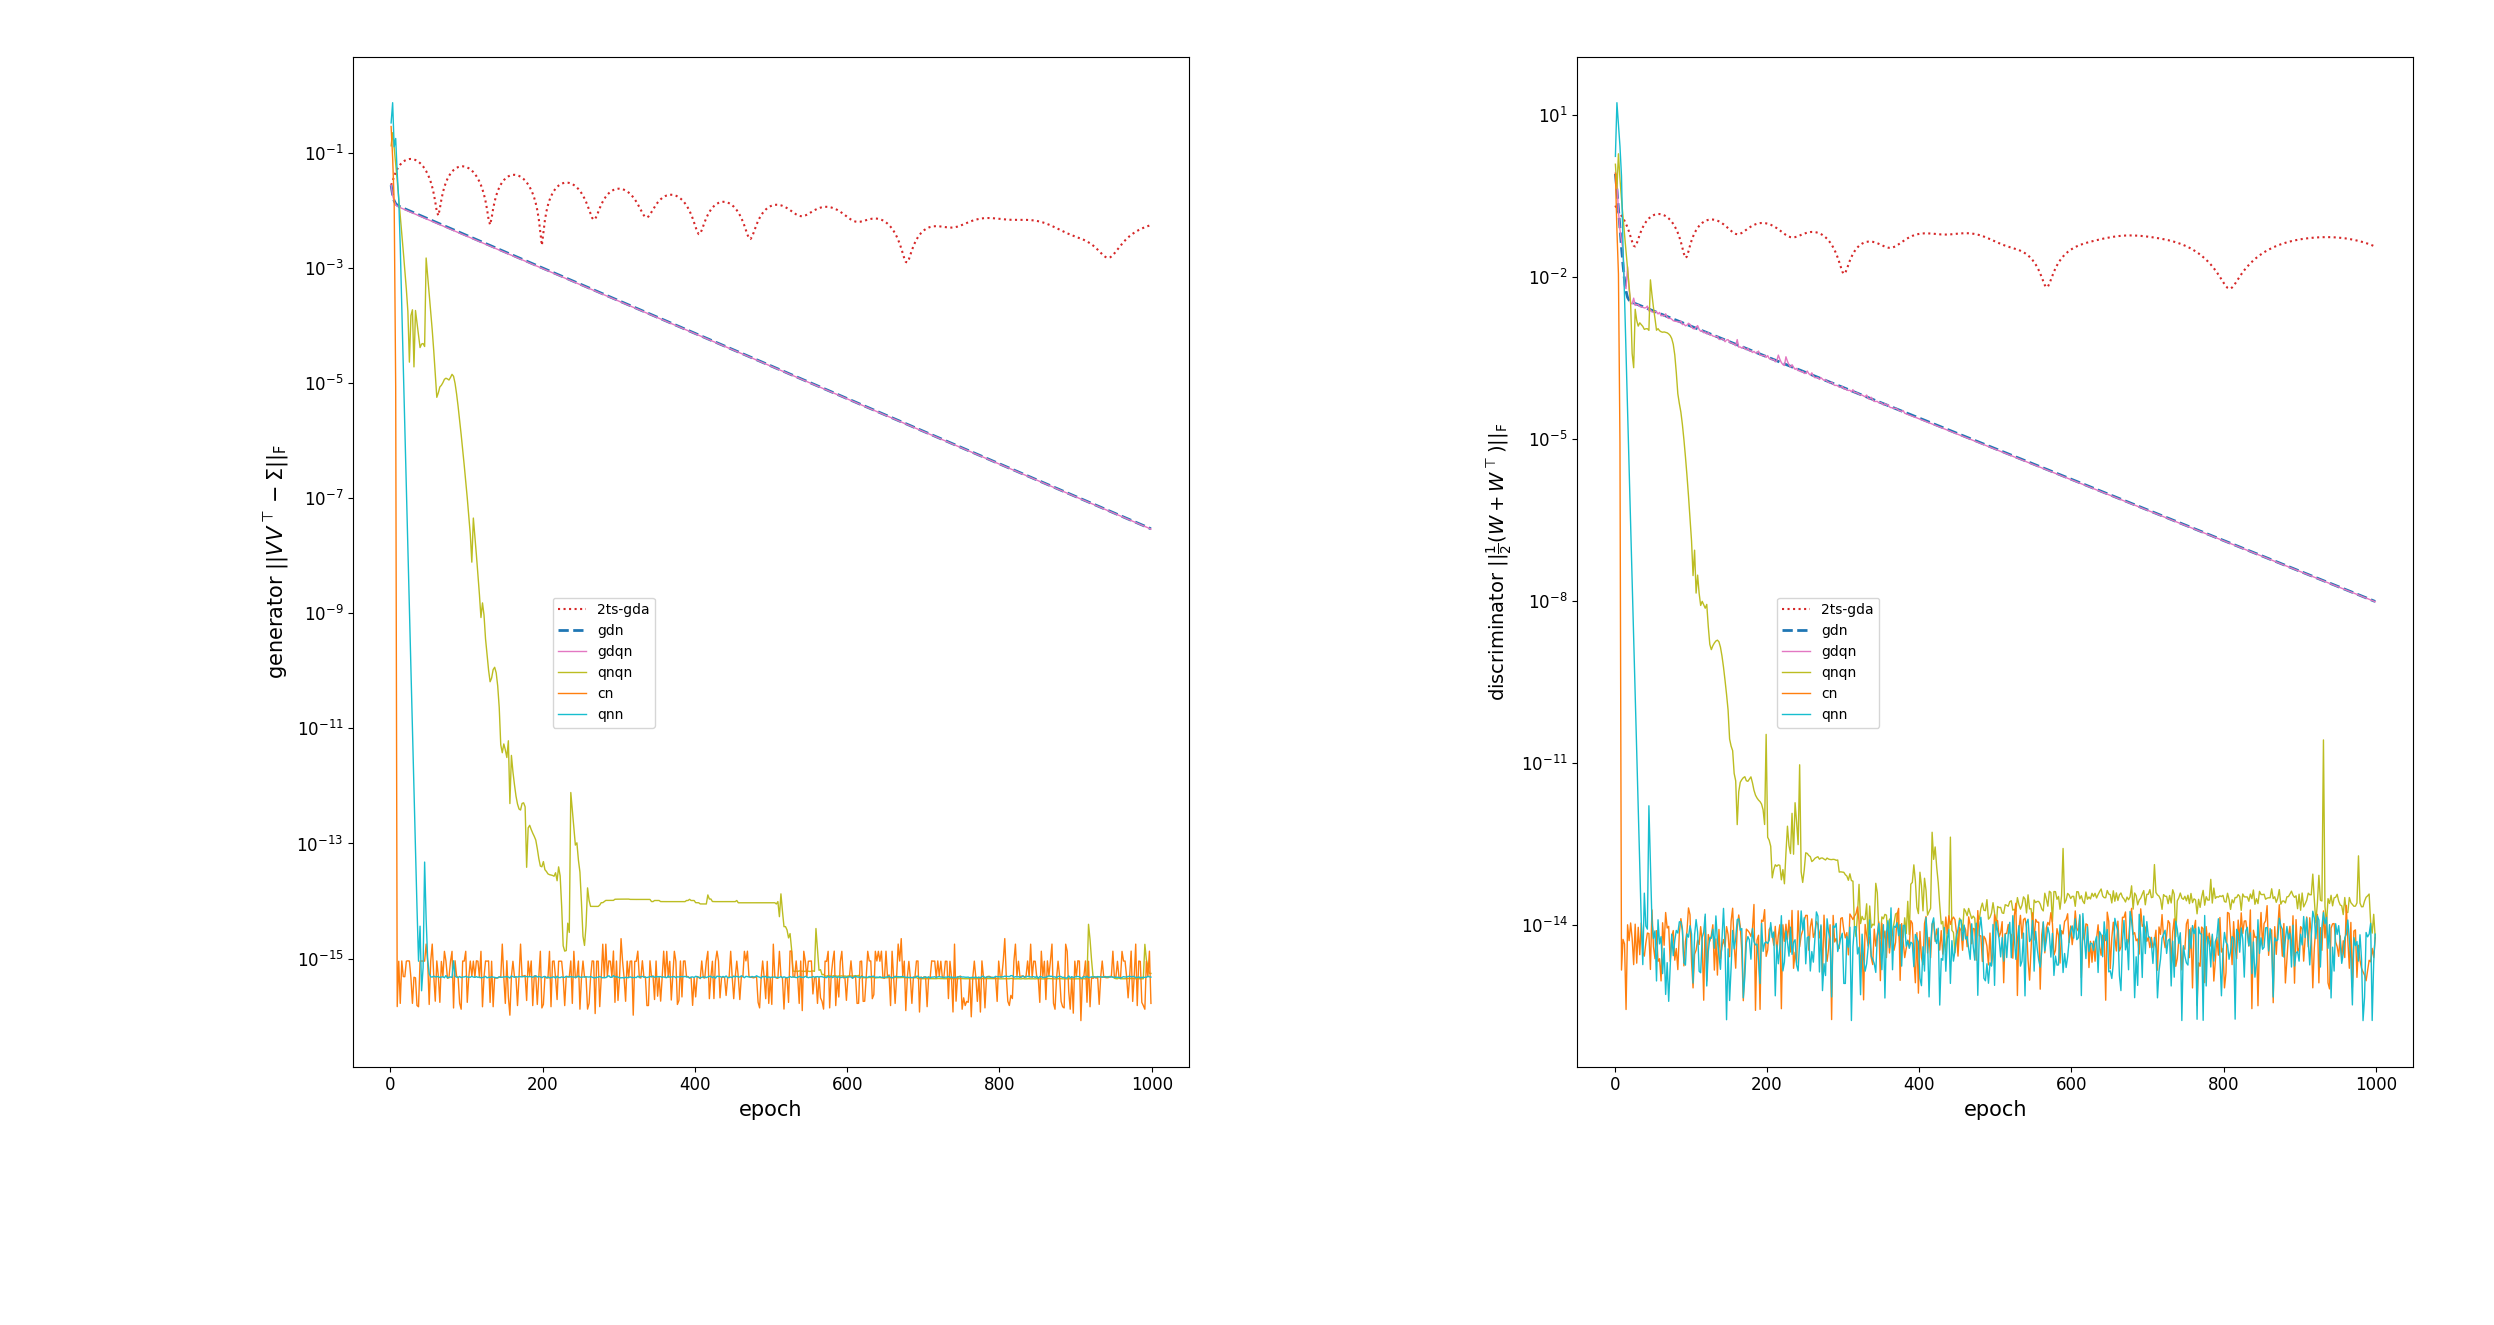
\includegraphics[width=\textwidth]{covariance_1000.png}
        \caption{Graph 1}
        \label{fig:graph1}
    \end{subfigure}
    \hfill
    \begin{subfigure}[b]{0.45\textwidth}
        \centering
        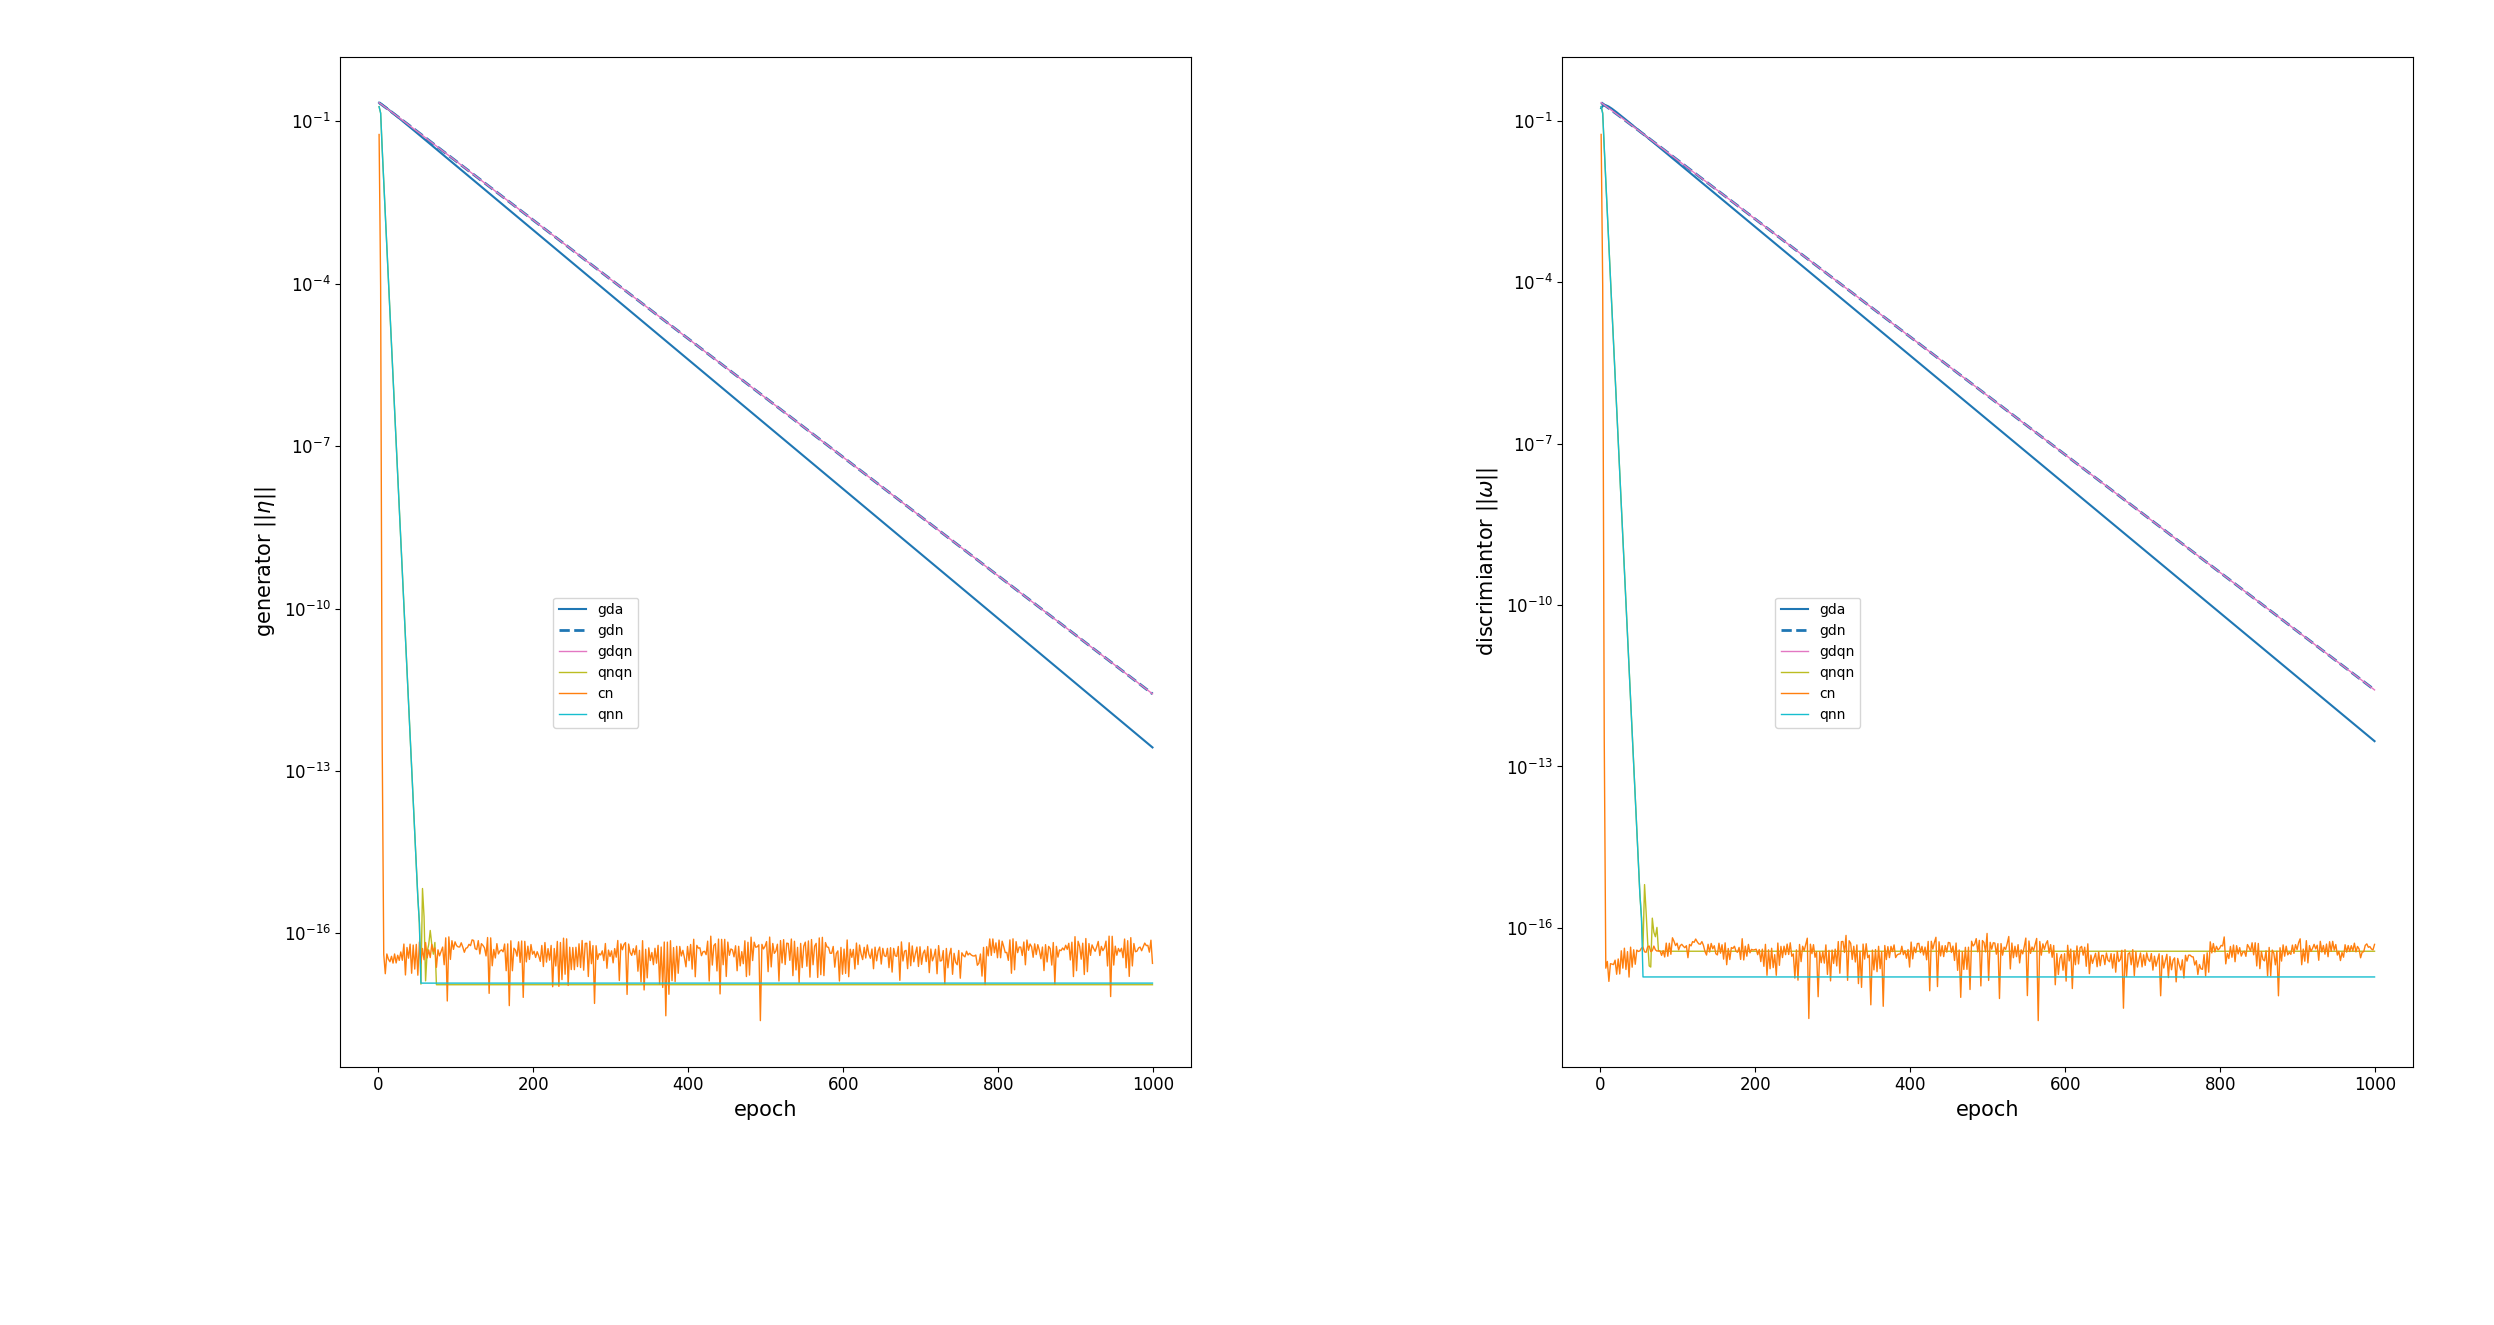
\includegraphics[width=\textwidth]{well_conditioned_guassian_mean_1000.png}
        \caption{Graph 2}
        \label{fig:graph2}
    \end{subfigure}

    \begin{subfigure}[b]{0.45\textwidth}
        \centering
        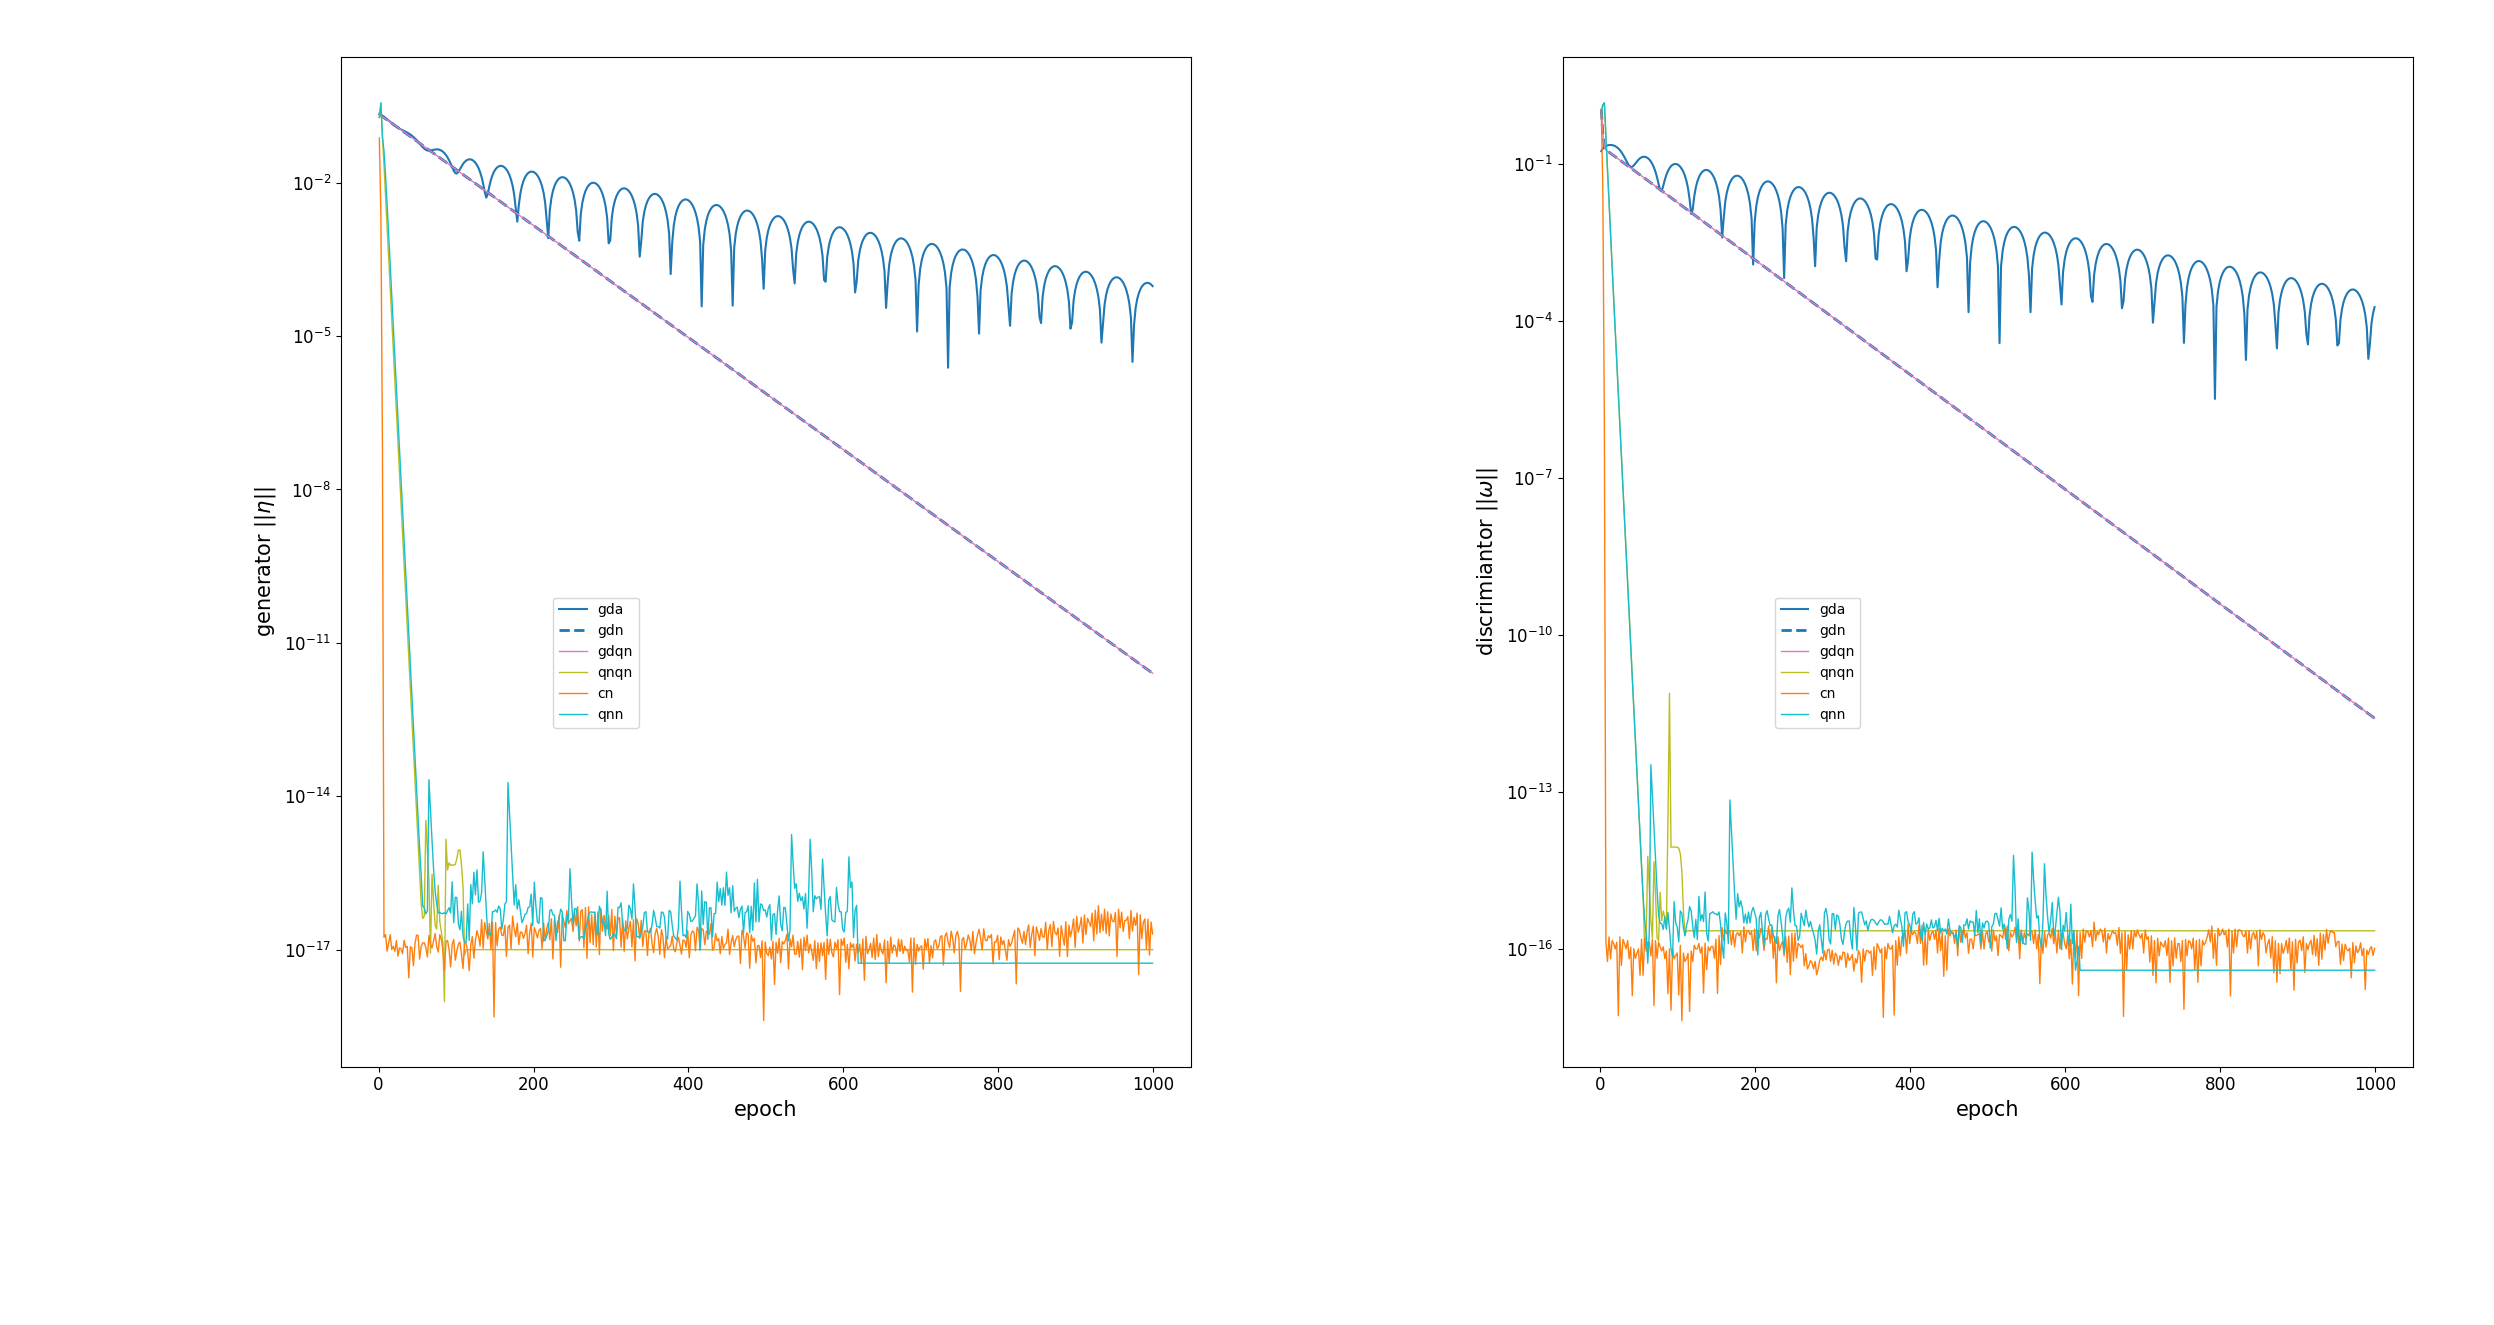
\includegraphics[width=\textwidth]{ill_conditioned_guassian_mean_1000.png}
        \caption{Graph 3}
        \label{fig:graph3}
    \end{subfigure}
    \hfill
    \begin{subfigure}[b]{0.45\textwidth}
        \centering
        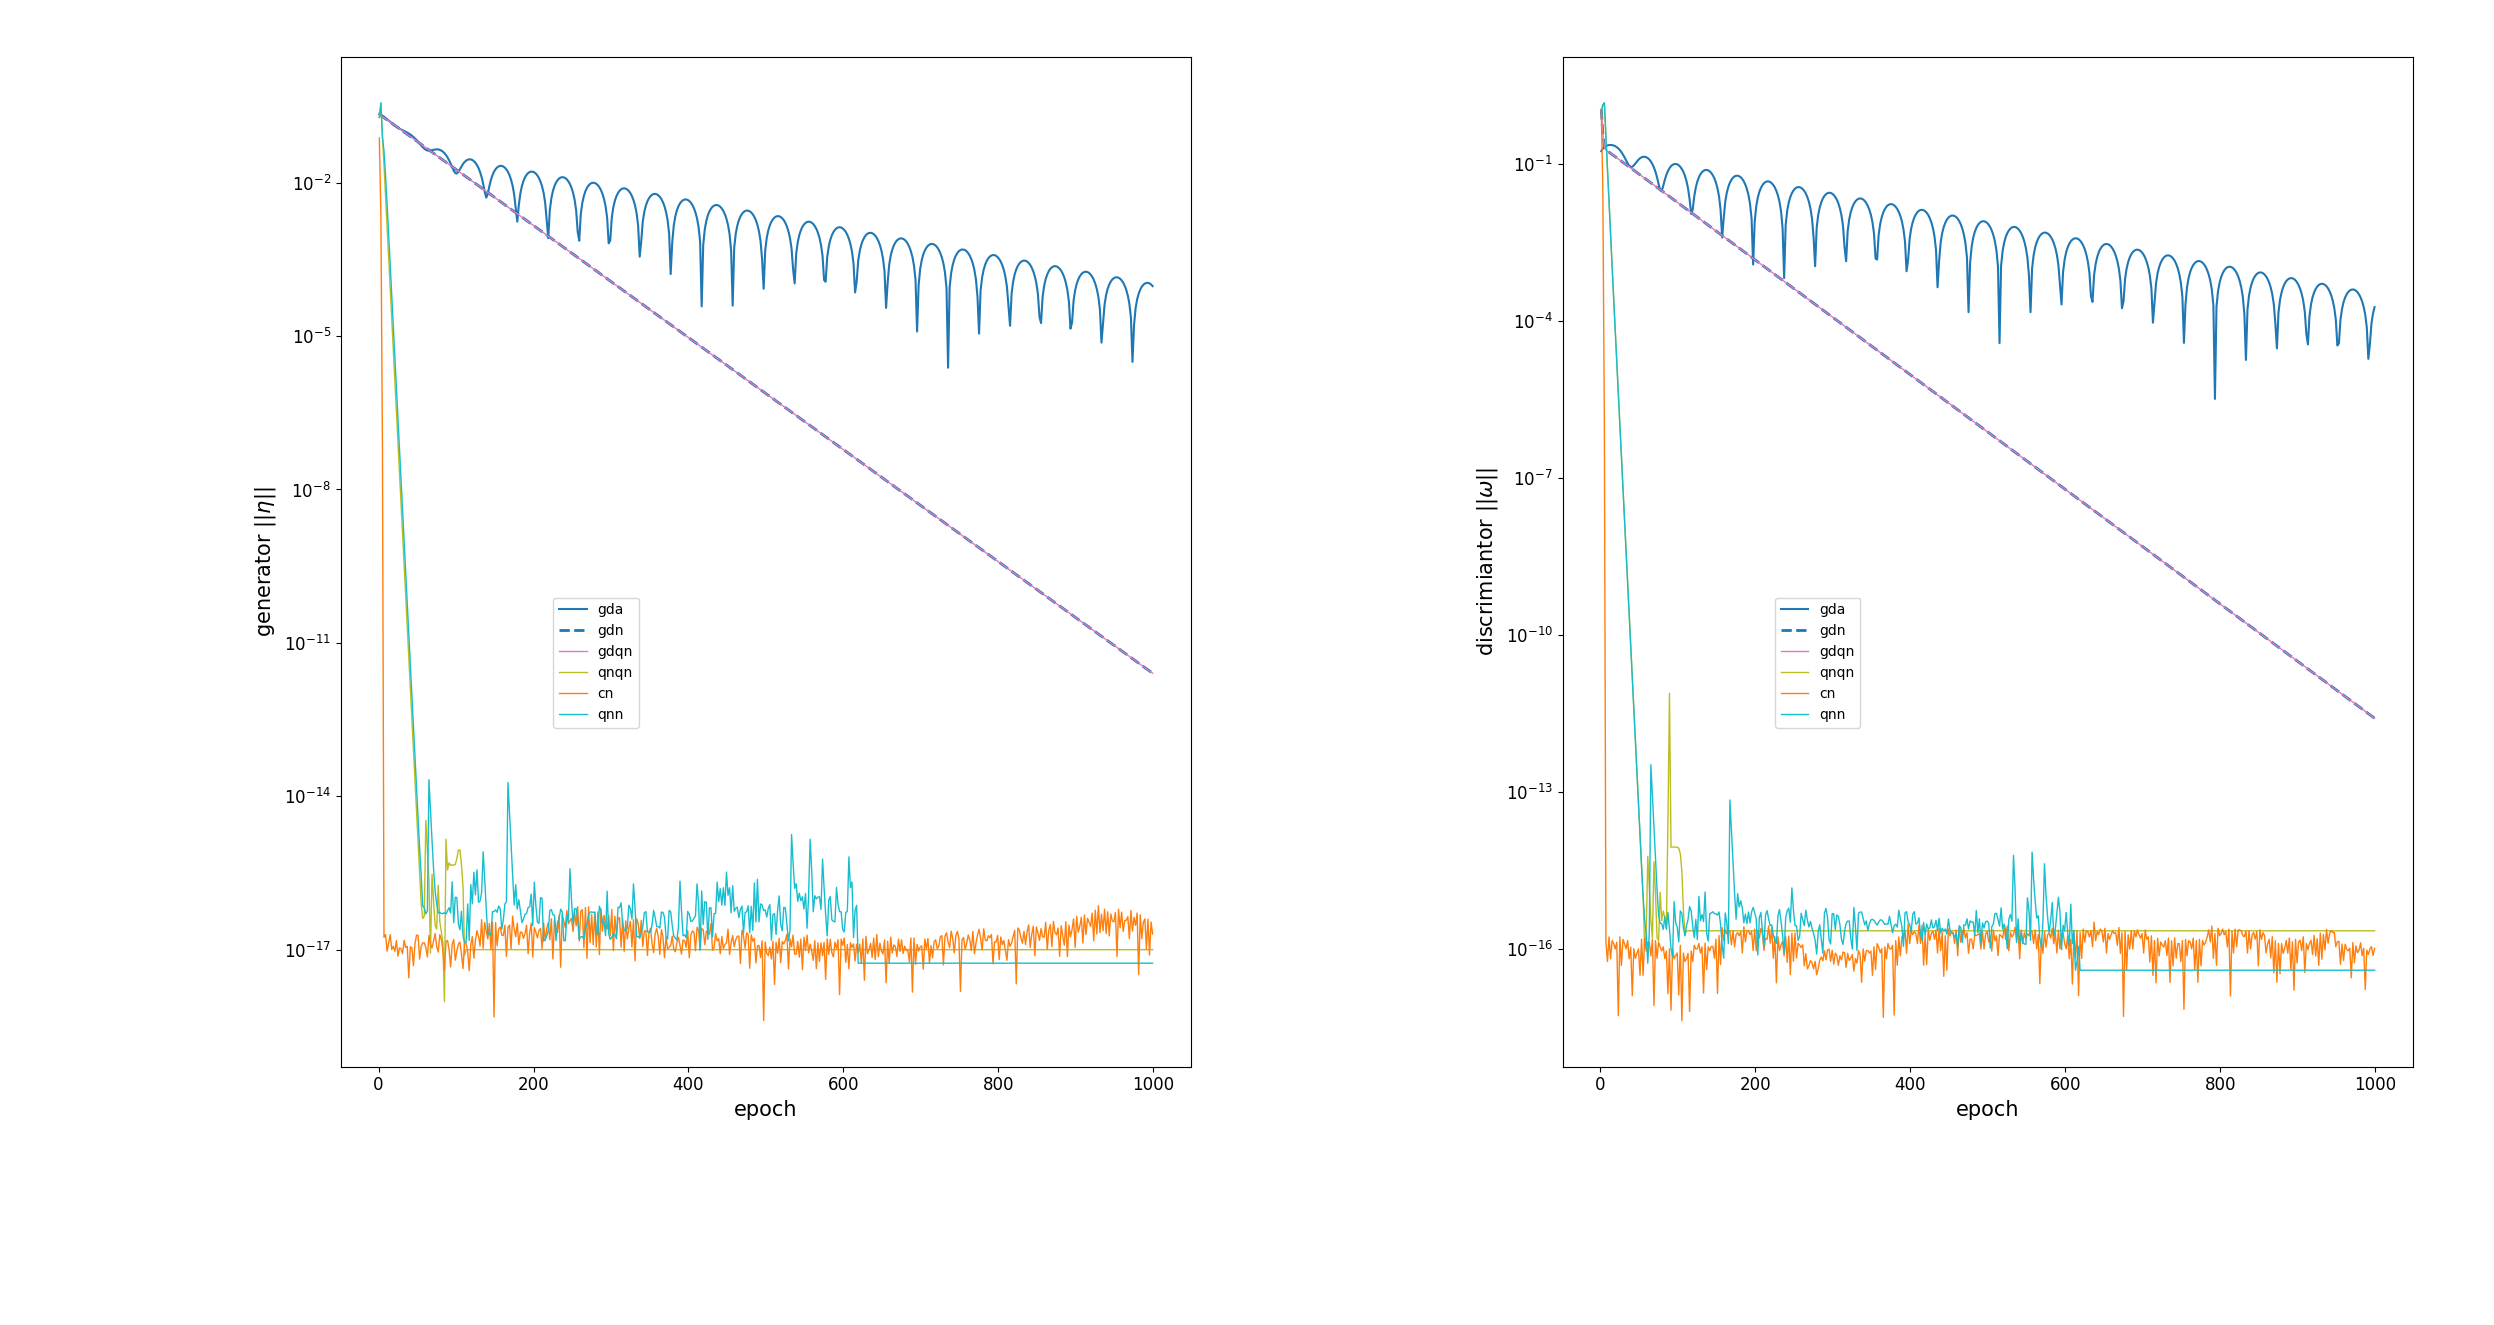
\includegraphics[width=\textwidth]{ill_conditioned_guassian_mean_1000.png}
        \caption{Graph 4}
        \label{fig:graph4}
    \end{subfigure}
    
    \caption{Multiple Graphs in One Figure}
    \label{fig:multiple_graphs}
\end{figure}

\subsection{well-conditioned guassian mean}
In well-conditioned guassian mean estimation, we have only 2 parameters for both generator and discriminator.
Our benchmark GDA converge linearly. GDN and GDBFGS also converge linearly perform a little bit worse than GDA while spending a little bit more time.
CBFGS and BFGSN converge superlinearly and CN converge even faster than CBFGS. However, CN do spend more time per epoch while CBFGS and BFGSN spends similar time to GDA, GDN and GDBFGS.

\subsection{ill-conditioned guassian mean}
In ill-conditioned guassian mean estimation, we also have only 2 parameters for both generator and discriminator.
The benchmark GDA start to perform weird.
The others algorithm have similar performance in well-conditioned one.
However, we can see that CN start spending more time compare to well-conditioned one.
Note: When using BFGS in training generator, we can't no longer use step size $\alpha_x = 1$ in this condition anymore, otherwise, it will diverge.

\subsection{covariance}
In guassian covariance estimation, we have 8 parameters for both generator and discriminator.
The benchmark GDA wasn't performing good.
GDN and GDBFGS still perform similarly and converge linearly. However Newton method start to spend more time then quasi-Newton method.
CN still converge the fastest but at the same time, it start to spend significantly more time then CBFGS (although still converge faster in time).
BFGSN have a performance really close to CN and only spend a little bit more time than CBFGS.
Note: Since the number of parameters increase, the time Newton method used increase significantly. However, we also need more steps to find $y^*$ to get close to the $\Phi(x)$ when using quasi-Newton method for inner problem.

\section{Future work}
\begin{itemize}
    \item try another midium scale problem (in J-symmetrix)
    \item try MNIST
    \item modify the condition number
\end{itemize}

\section{Other Note}
\begin{itemize}
    \item generator is the minimizer which is the slow leader
    \item discriminator is the maximizer which is the faster follower
    \item I think the paper take a trick on gradient step, make the step size smaller(0.05 for outer, 0.5 for inner), so the performance of Newton type method become better.
    \item Finish LBFGS update.
    \item size 100: CN perform the best.
\end{itemize}

\section{Outline}
\begin{itemize}
    \item Introduation
    \begin{itemize}
        \item application of minimax problem
        \item basic idea of solving minimax problem
        \item mention uzawa's approach
        \item talk about gradient based method and Newton method
        \item talk about quasi-Newton method
    \end{itemize}
    \item Preliminary
    \begin{itemize}
        \item introduce minimax problem
        \item introduce SLmM
        \item analyze the gradient around SLmM
    \end{itemize}
\end{itemize}

\bibliographystyle{plain}
\bibliography{reference}

\end{document}